\section{SMART Goal 3: Test of DQM Tooling}
This smart goal follows the test of the designated DQM tool with which a test leading up to a master thesis can be performed. The usecase was defined during a call with a solution architect as described in the previous section. It uses one deliverable of the AWS modernisation, which is a monitoring for jobs. However the monitoring was also designed in a way that some data could be checked. However this functionality was developed only in a very basic way, so it had to be confirmed that it is fit to handle checks as they would be used during the master thesis.

\subsection*{Knowledge transfer sessions}
As the AWS modernisation team was developing the functionality, in turn knowledge transfer sessions were held to show the \gls{DWHLSOPS} team how to use it. Furthermore extensive documentation was written describing the interlinkage of the different \gls{awsService}


\begin{figure}[H]
    \centering
    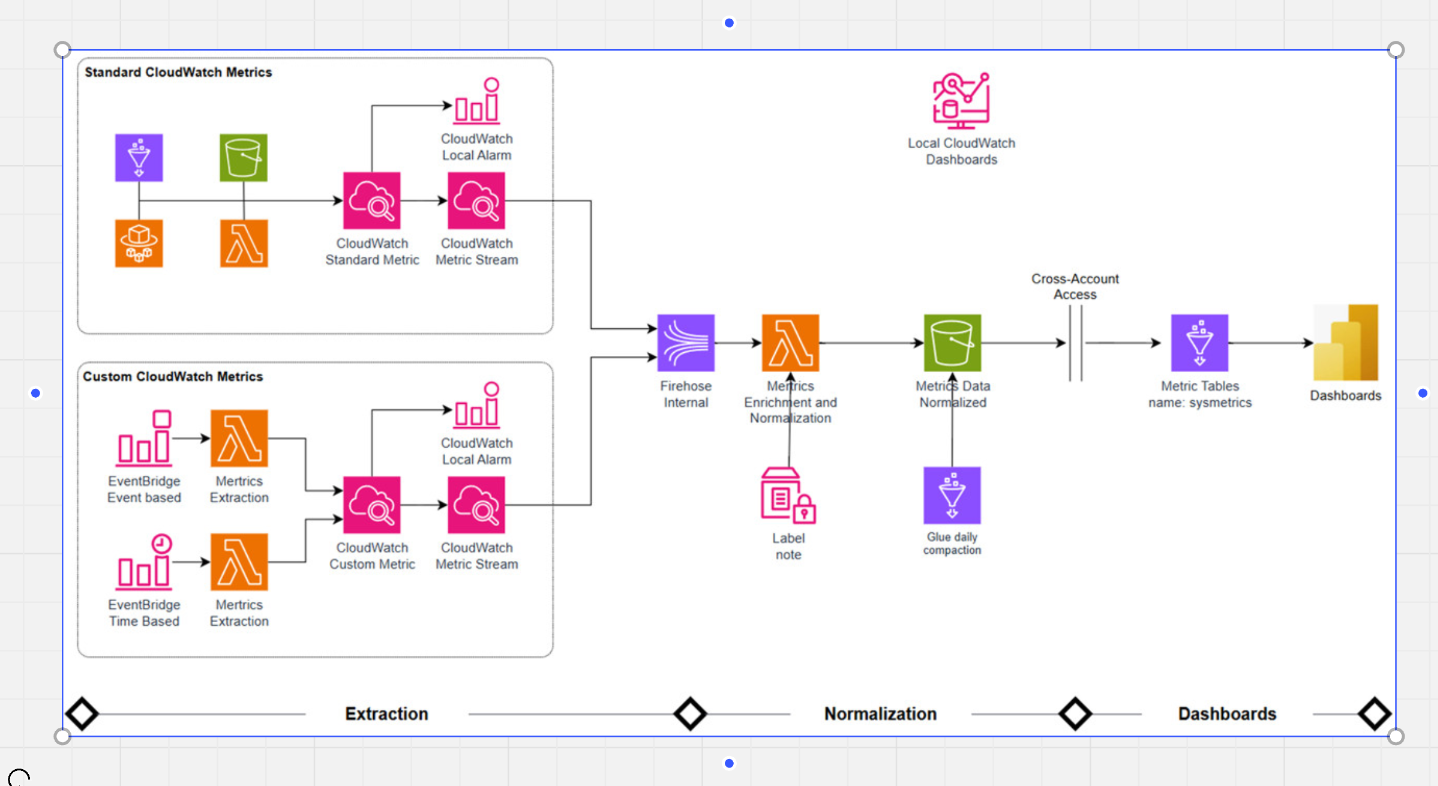
\includegraphics[width=0.95\textwidth]{./content/img/AWS_Monitoring_Architecture.png}
    \caption{AWS monitoring architecture showing the extraction, normalization, and dashboarding pipeline implemented using AWS services}
    \label{fig:aws_monitoring_architecture}
\end{figure}

\subsection*{First steps creating view for testing}



\subsection*{creating new resources}





Was das Diagramm erklärt

Der Prozess beginnt mit den Entwicklungswerkzeugen:

State the obvious!
Entwicklung erfolgt mit JetBrains IntelliJ IDEA.
Die Infrastruktur bzw. Konfiguration wird mit Terraform verwaltet.

Von dort wird der eigentliche Entwicklungsprozess beschrieben:

Als Versionsverwaltung wird Git (Bitbucket) verwendet.
Für Änderungen müssen die Regeln zum Erstellen von Branches eingehalten werden.
Der Entwickler arbeitet auf einem eigenen Branch (mittig ist als Beispiel ein git status auf einem Feature-Branch dargestellt).
Sobald die Änderung fertig ist, muss ein Pull Request erstellt werden.
Anschließend erfolgt der Merge in den Master-Branch.
Vor dem Merge ist ein Test Build erforderlich.
Für die Entwicklungsumgebung (Dev) reicht ein erfolgreicher Build aus, damit der Merge durchgeführt werden kann.
Was noch ergänzt werden könnte

Im Vergleich zu deinem ersten Diagramm fehlen hier noch einige Informationen, die den Prozess vollständiger machen würden:

Wer überprüft den Pull Request?
Ist mindestens ein Review erforderlich?
Gibt es unterschiedliche Anforderungen zwischen Dev und Prod?
Wird nach dem Merge automatisch deployed oder manuell?
Gibt es mehrere Repositories (Test / Production)?
Erfolgt der Build über eine CI/CD-Pipeline?

Gerade diese Punkte wären für einen wissenschaftlichen Bericht interessant, da sie den organisatorischen Teil des DevOps-Prozesses beschreiben.

Wie man das wissenschaftlicher beschreiben könnte

Anstatt die einzelnen Werkzeuge aufzuzählen, würde ich den Ablauf eher prozessorientiert beschreiben, beispielsweise:

Infrastructure changes are implemented using Terraform within the IntelliJ IDEA development environment. Source code is managed using Git with Bitbucket as the central repository. Each change is developed on a dedicated feature branch following the project's branching conventions. After implementation, a pull request is created and submitted for integration into the master branch. Before the merge can be completed, a successful build must be executed. For the development environment, a successful build is sufficient to allow the merge.


\subsection*{final stuff..... new resources}

Die Notizen dokumentieren im Grunde einen Proof of Concept (PoC) zur Einführung einer ersten Data-Quality-Metrik innerhalb der AWS-Monitoring-Architektur. Es geht weniger um die technische Implementierung selbst, sondern darum, den gesamten Prozess von der Definition bis zur erfolgreichen Ausführung einer Metrik zu validieren.

Inhalt der Notizen
Ziel
Query zur Überwachung erstellen.
Prüfen, ob das definierte Monitoring mit dieser Query funktioniert.
Hinterfragen, ob die Query in der vorgesehenen Form umgesetzt werden sollte.
Gefundener Fehler

Während der Validierung wurde ein Problem festgestellt:

Fehler in der AWS-Umgebung (Canbda).
Gemeinsam mit einer Kollegin (Kristina) überprüft.
Ursache war ein Copy-and-Paste-Fehler.
Falscher Wert:
HRK = 014
Richtiger Wert:
LocationKey = HRK
Umsetzung
Fehler wurde korrigiert.
Dafür musste ein weiterer Pull Request erstellt werden.
Ergebnis
Die Metrik wurde anschließend erstmals erfolgreich ausgeführt.
Zeitpunkt:
10:45 CEST, 11.05.2026
Erkenntnisse

Eine wichtige Erkenntnis ist am Ende notiert:

Jede zusätzliche Monitoring-Metrik verursacht laufende Kosten, da mehrere AWS-Services beteiligt sind, beispielsweise

AWS Lambda
Amazon CloudWatch
Amazon S3

Deshalb sollten Test- oder PoC-Metriken nach Abschluss der Validierung möglichst zeitnah wieder entfernt werden.

Wie würde ich das in SMART Goal 3 beschreiben?

Ich würde die Notizen nicht als "Meeting Notes" oder "Personal Notes" darstellen, sondern als Dokumentation der ersten Validierung des Monitoring-Konzepts.

Beispielsweise:

As preparation for the Master's thesis, an initial proof of concept was conducted to validate the proposed AWS-based data quality monitoring architecture. This included defining an initial monitoring query, deploying the corresponding metric, validating its execution, and troubleshooting configuration issues encountered during the implementation. During this process, a configuration error caused by an incorrect mapping was identified and resolved through an additional pull request. After the correction, the monitoring metric was successfully executed for the first time. The proof of concept also demonstrated that each monitoring metric introduces operational costs through the involved AWS services, highlighting the importance of removing temporary test metrics after validation.

Warum das gut zu SMART Goal 3 passt

SMART Goal 3 lautet sinngemäß, die Werkzeuge und die technische Machbarkeit für die spätere Masterarbeit vorzubereiten. Genau das zeigen diese Notizen:

erste praktische Validierung der Architektur,
Implementierung einer Monitoring-Metrik,
Behebung eines realen Implementierungsfehlers,
erfolgreicher Nachweis der Funktionsfähigkeit,
Erkenntnisse über betriebliche Auswirkungen (Kosten).

Das macht aus den handschriftlichen Notizen einen nachvollziehbaren Validierungsschritt innerhalb deines Projekts und nicht nur eine Sammlung persönlicher Arbeitsnotizen.

Oder etwas allgemeiner:

The DevOps workflow follows a standard Git-based development process. Developers implement infrastructure changes using Terraform, commit their work to feature branches, and submit pull requests for integration into the main branch. Automated build validation ensures that only successfully verified changes are merged into the development environment.